\documentclass[10pt,twocolumn,a4paper]{article}
\usepackage[a4paper,top=0.75in,bottom=1.0in,left=0.68in,right=0.68in,columnsep=0.25in]{geometry}
\usepackage{mathptmx}
\usepackage[T1]{fontenc}
\usepackage[utf8]{inputenc}
\usepackage{graphicx}
\usepackage{amsmath,amssymb}
\usepackage{booktabs}
\usepackage{array}
\usepackage{titlesec}
\usepackage{caption}
\usepackage{cite}
\usepackage[hidelinks]{hyperref}
\usepackage{url}
\renewcommand{\thesection}{\Roman{section}}
\renewcommand{\thesubsection}{\Alph{subsection}}
\titleformat{\section}[block]{\centering\normalsize\scshape}{\thesection.}{0.5em}{}
\titleformat{\subsection}[block]{\normalsize\itshape}{\thesubsection.}{0.5em}{}
\titlespacing*{\section}{0pt}{1.4ex plus 1ex minus .2ex}{1ex}
\titlespacing*{\subsection}{0pt}{1.0ex plus 1ex minus .2ex}{0.6ex}
\newcommand{\abstractkw}[1]{\noindent\textbf{\textit{#1}}}
\captionsetup{font=small,labelsep=period}
\setlength{\parindent}{1em}
\setcounter{topnumber}{3}
\renewcommand{\topfraction}{0.9}
\renewcommand{\textfraction}{0.05}

\begin{document}
\twocolumn[
\begin{@twocolumnfalse}
\begin{center}
{\LARGE\bfseries From-Scratch Decision Trees and Pegasos SVM\\for Bina.az Real-Estate Modelling\par}
\vspace{1.0em}
{\large Samir Hasanov,\quad Mammadaliyev Ramil,\quad Elmin Seyidov\par}
\vspace{0.4em}
{\itshape MLE-AI-201 Machine Learning, AI Academy --- Cohort II\par}
\vspace{1.0em}
\end{center}
\begin{quote}\small
\abstractkw{Abstract---}
We study 100,775 Bina.az sale records as two supervised tasks: sale-price regression and price-tier classification. After deduplicating repeated listing snapshots and applying fixed plausibility rules, 64,128 listings remain. We build 29 numeric features and implement a decision tree in NumPy for both tasks, plus a linear Pegasos SVM and a random Fourier feature (RFF) extension for classification. The premium threshold of 210,000 AZN and SVM scaling statistics come from training data only; model settings are chosen on validation data. On the held-out test set, our tree classifier reaches F1=0.9099 and ROC-AUC=0.9630, close to scikit-learn's tree (F1=0.9103). Linear Pegasos reaches F1=0.8228, while RFF lowers it to 0.8101. The regression tree reaches RMSE=310,716 AZN and $R^2=0.5921$. Classification is strong, but price errors remain large for the most expensive listings. These results show that the hand-built models are useful learning baselines, while remaining sensitive to model choice and the long-tailed target. Submission repository: \url{https://github.com/Hasanov57/Bina.az_ML_Final_Project} (planned tag \texttt{v1.0-final}).

\vspace{0.5em}
\abstractkw{Index Terms---}decision tree, SVM, Pegasos, random Fourier features, regression, classification, real estate.
\end{quote}
\vspace{0.8em}
\end{@twocolumnfalse}
]
\small

\section{Introduction}
Real-estate price modelling is a useful test of machine-learning fundamentals because prices depend on interacting structural and geographic variables and real listing data is noisy. This project uses the Bina.az sale dump~\cite{dataset} to study two tasks: predicting sale price and predicting whether a listing belongs to a premium price tier. Our main contributions are: (1) a reproducible cleaning and feature pipeline, (2) a from-scratch NumPy decision tree supporting regression and classification, (3) a from-scratch soft-margin SVM trained with Pegasos plus a random Fourier feature extension, and (4) matched comparisons against scikit-learn~\cite{sklearn} with validation curves, uncertainty estimates, feature analysis, and error analysis.

\section{Background}
A decision tree recursively chooses a feature and threshold that maximally decreases node impurity. For classification we implement Gini impurity and entropy; for regression we use variance/MSE reduction. Leaves predict the majority class or the mean target value. Tree complexity is controlled by maximum depth, minimum split size, minimum leaf size, and minimum impurity decrease.

For binary classification, the soft-margin SVM minimises regularised hinge loss. We use the Pegasos stochastic sub-gradient method~\cite{pegasos} rather than a QP/SMO solver. At update step $t$, the learning rate is $\eta_t=1/(\lambda t)$. If a sampled point violates the margin, its labelled feature vector contributes to the update; otherwise only regularisation shrinkage is applied. Features are standardised from training statistics. For non-linearity, we approximate an RBF kernel with random Fourier features (RFF) and apply the same linear Pegasos solver in the mapped space.

\section{Data and Preprocessing}
The raw CSV contains 100,775 rows and 51 columns. Many rows are repeated snapshots of the same listing. We sort snapshots by scrape time and retain the latest record per listing URL, then apply fixed plausibility filters for obvious entry/scrape errors (for example 11 AZN listings, 600M AZN listings, and 200,000 m$^2$ area values). This produces 64,128 unique cleaned listings.

We parse floor area, room count, current/total floor, land area, latitude and longitude into numeric values. Missing room/floor/land values are encoded as zero with explicit missing indicators, avoiding medians learned from validation/test data. Low-cardinality category and city columns are one-hot encoded. Repair, deed and mortgage availability are encoded as binary variables. High-cardinality identifiers, raw URLs, names, addresses and free text are not used in the core model. Critically, \texttt{unit\_price} and \texttt{total\_price} are removed because they are arithmetic functions of the target and would cause target leakage.

We first select the 70\% training split. The price-tier threshold is then the median of training prices only: 210,000 AZN. The remaining observations are divided into 15\% validation and 15\% test sets with tier stratification. The final split sizes are 44,890 / 9,619 / 9,619, with premium proportions 0.496 / 0.494 / 0.494. Scaling for the SVM uses training means and standard deviations only.

Exploration shows a strongly right-skewed price distribution. Larger area generally accompanies higher price, but listings of similar size still vary widely. The training-median tier definition yields near-balanced classes.

\begin{table}[t]
\centering
\caption{Dataset summary after cleaning.}
\label{tab:data}
\begin{tabular}{@{}lr@{}}
\toprule
Property & Value \\
\midrule
Raw rows & 100,775 \\
Clean unique listings & 64,128 \\
Features & 29 \\
Train / Val / Test & 44,890 / 9,619 / 9,619 \\
Premium threshold & 210,000 AZN \\
Premium share: train / val / test & 49.6\% / 49.4\% / 49.4\% \\
\bottomrule
\end{tabular}
\end{table}

\section{Method}
\subsection{Decision Tree}
For each numeric feature we sort values and evaluate candidate thresholds between adjacent distinct values. The best split maximises
\begin{equation}
\Delta I=I(P)-\frac{N_L}{N}I(L)-\frac{N_R}{N}I(R).
\end{equation}
Classification impurity is either $1-\sum_k p_k^2$ (Gini) or $-\sum_k p_k\log_2 p_k$ (entropy). Regression impurity is node variance. The implementation recursively creates child nodes until a stopping condition is met. Leaf class probabilities are empirical class frequencies, and feature importance is accumulated weighted impurity decrease. A toy deterministic dataset is checked against scikit-learn; the root feature, threshold and predictions match.

\subsection{Pegasos SVM and RFF}
The linear SVM minimises
\begin{equation}
J(\mathbf{w},b)=\frac{\lambda}{2}(\lVert\mathbf{w}\rVert^2+b^2)+\frac1n\sum_i\max(0,1-y_i(\mathbf{w}^T\mathbf{x}_i+b)).
\end{equation}
Labels are mapped to $\{-1,+1\}$. A constant feature folds the bias into the update, followed by the standard Pegasos L2-ball projection. The objective includes the bias penalty used by this augmented update, so the logged values and convergence curve represent the same function as training. Support vectors are training observations satisfying $y_i f(x_i)\leq 1$. For the final linear model, $\lVert\mathbf{w}\rVert=5.979$, margin width $2/\lVert\mathbf{w}\rVert=0.335$, and 19,892 of 44,890 training listings are on or inside the margin. The RFF extension samples random frequencies corresponding to an RBF kernel and maps each input to cosine features before applying Pegasos.

\section{Experimental Setup}
Regression trees are trained on $\log(1+price)$ because the price distribution is strongly right-skewed; predictions are exponentiated for price-scale RMSE, MAE and $R^2$. Classification uses precision, recall, F1 and ROC-AUC. All random seeds are fixed to 42.

Validation data only is used to select hyperparameters. Regression depth is swept over 4, 6, 8, 10 and 12, followed by minimum-leaf sizes 5, 20, 50 and 100. Classification compares Gini against entropy, then sweeps depth and minimum-leaf size. Pegasos sweeps $\lambda\in\{10^{-2},3\times10^{-3},10^{-3},3\times10^{-4}\}$, epochs $\in\{1,2,3,5\}$, and three learning-rate schedules (Pegasos $1/(\lambda t)$, inverse-square-root, and constant). RFF sweeps $\gamma\in\{0.03,0.1,0.3\}$. The selected configurations are regression tree depth 12/leaf 5, classification tree Gini/depth 11/leaf 5, linear SVM $\lambda=10^{-3}$ with 3 epochs and the Pegasos schedule, and RFF $\gamma=0.1$ with 120 components. Baselines are scikit-learn decision trees and a \texttt{StandardScaler + SGDClassifier(loss='hinge')} pipeline.

\section{Results}
\begin{table}[t]
\centering
\caption{Held-out price regression results (AZN).}
\label{tab:regresults}
\begin{tabular}{@{}lrrr@{}}
\toprule
Model & RMSE & MAE & $R^2$ \\
\midrule
Our Tree & 310,716 & 87,181 & 0.5921 \\
Sklearn Tree & 299,329 & 86,475 & 0.6215 \\
\bottomrule
\end{tabular}
\end{table}

\begin{table}[t]
\centering\scriptsize
\caption{Held-out Premium classification results.}
\label{tab:clsresults}
\begin{tabular}{@{}lrrrr@{}}
\toprule
Model & Precision & Recall & F1 & AUC \\
\midrule
Our Tree & 0.9059 & 0.9139 & 0.9099 & 0.9630 \\
Sklearn Tree & 0.9068 & 0.9139 & 0.9103 & 0.9629 \\
Linear Pegasos & 0.8439 & 0.8027 & 0.8228 & 0.9083 \\
RFF Pegasos & 0.8141 & 0.8061 & 0.8101 & 0.8936 \\
Sklearn SGD & 0.8457 & 0.8069 & 0.8259 & 0.9077 \\
\bottomrule
\end{tabular}
\end{table}

For classification, the from-scratch tree is nearly indistinguishable from the library implementation on F1/AUC, indicating that split search, stopping rules and leaf predictions are behaving correctly. The linear SVM is weaker, consistent with a problem where location, area and property type interact non-linearly. The RFF extension did not improve F1 under the tested dimensionality/bandwidth settings.

Three-fold cross-validation on a fixed-seed 18,000-row subset of the development data provides a practical uncertainty estimate without using the final test set. Mean $\pm$ standard deviation F1 is $0.8949\pm0.0054$ for our tree, $0.8970\pm0.0062$ for the sklearn tree, $0.8216\pm0.0096$ for linear Pegasos, $0.8099\pm0.0031$ for RFF Pegasos, and $0.8324\pm0.0013$ for sklearn's hinge-loss pipeline. Regression RMSE is $364,775\pm21,116$ AZN for our tree and $364,667\pm21,064$ AZN for the sklearn tree. The subset is used only to keep repeated from-scratch tree fitting computationally practical.

The SVM controls have visible effects. With $\lambda=10^{-3}$ and the Pegasos schedule, validation F1 changes from 0.8224 after one epoch to 0.8330 after three epochs, while the margin width changes from 0.241 to 0.335. At three epochs, Pegasos, inverse-square-root, and constant schedules obtain F1 values 0.8330, 0.8000, and 0.8204 with margin widths 0.335, 0.789, and 0.437 respectively. Thus the epoch count and learning-rate schedule change both the learned separator and its margin.

\begin{table}[t]
\centering
\caption{Representative fit and prediction timing from the current results file.}
\label{tab:timing}
\begin{tabular}{@{}lrr@{}}
\toprule
Model & Fit (s) & Predict (ms/1000) \\
\midrule
Our Tree Classifier & 1.32 & 5.03 \\
Sklearn Tree Classifier & 0.18 & 0.36 \\
Our Linear Pegasos & 1.06 & 0.070 \\
Our RFF Pegasos & 1.27 & 2.54 \\
Sklearn SGD pipeline & 0.36 & 0.40 \\
\bottomrule
\end{tabular}
\end{table}

A separate fixed-seed scaling experiment with 2k, 5k and 10k training rows shows fit time increasing with sample size for both models; the from-scratch tree grows from about 0.12 s to 0.43 s, while linear Pegasos grows from about 0.05 s to 0.24 s. Timing depends on machine load.

\begin{table}[t]
\centering\scriptsize
\caption{Test confusion matrices (Premium is positive).}
\label{tab:confusion}
\begin{tabular}{@{}lrrrr@{}}
\toprule
Model & TN & FP & FN & TP \\
\midrule
Our Tree & 4,419 & 451 & 409 & 4,340 \\
Linear Pegasos & 4,165 & 705 & 937 & 3,812 \\
\bottomrule
\end{tabular}
\end{table}

\begin{figure}[t]
\centering
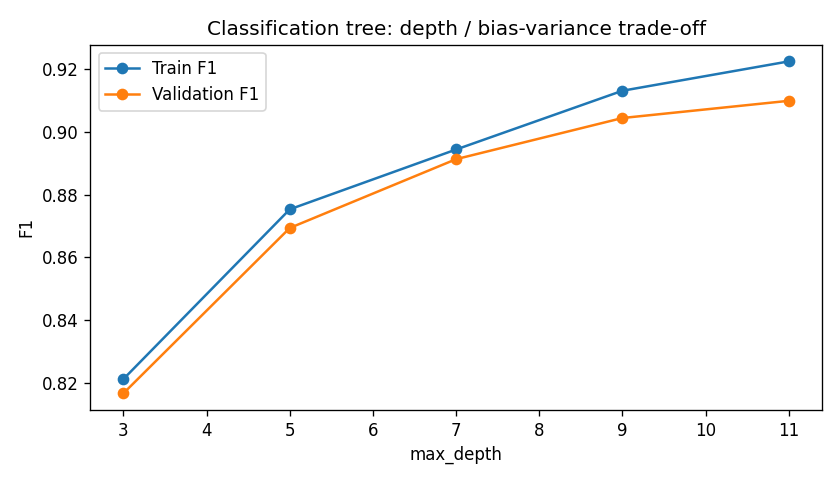
\includegraphics[width=\linewidth]{figures/tree_classification_depth_sweep.png}
\caption{Train and validation F1 both rise over tested depths. The gap widens slightly, but validation F1 does not fall.}
\label{fig:depth}
\end{figure}

\begin{figure}[t]
\centering
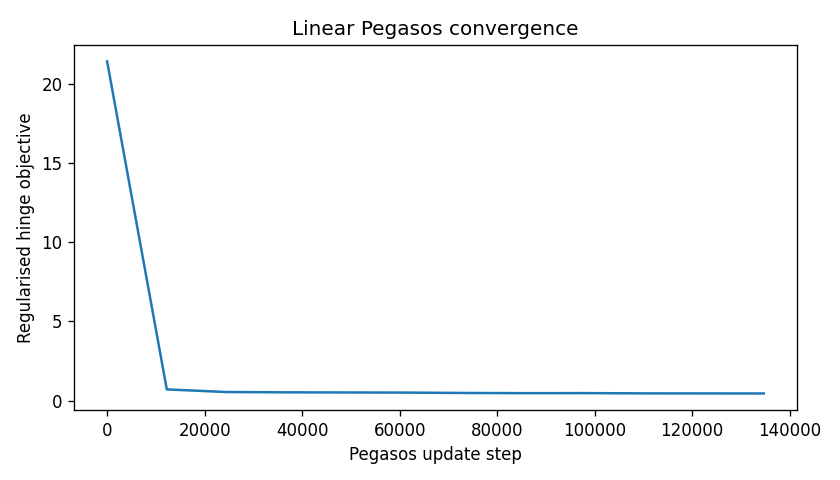
\includegraphics[width=\linewidth]{figures/svm_convergence.png}
\caption{The recorded augmented-vector hinge-loss objective falls quickly and then stabilises.}
\label{fig:svmconv}
\end{figure}

\begin{figure}[t]
\centering
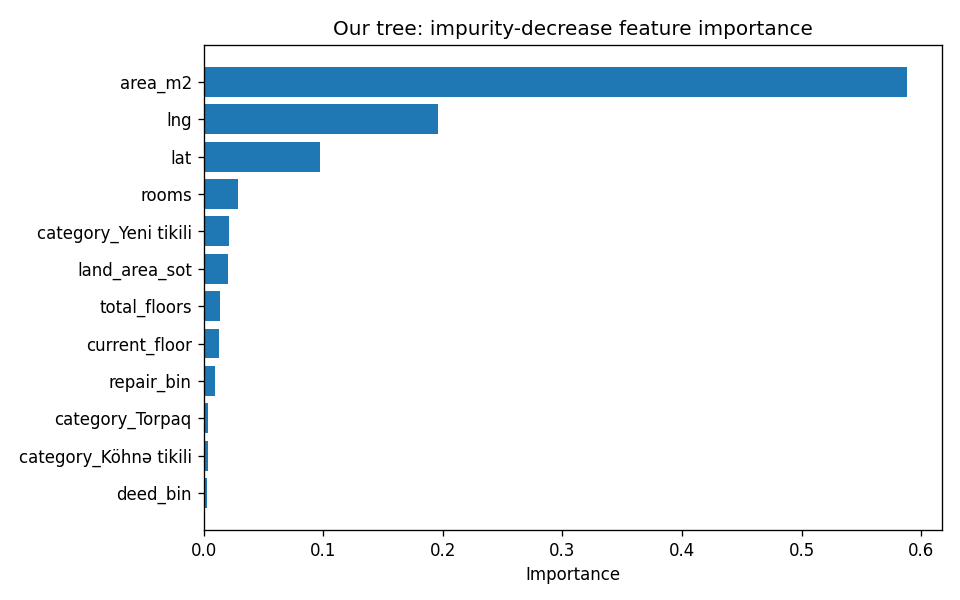
\includegraphics[width=\linewidth]{figures/tree_feature_importance.png}
\caption{Impurity-decrease importance of the final from-scratch classification tree.}
\label{fig:importance}
\end{figure}

\section{Discussion and Limitations}
The tree relies most heavily on area (58.8\% of impurity-decrease importance), longitude (19.6\%) and latitude (9.8\%). These scores describe this fitted model; they do not establish causal effects. Room count, new-build status, land area and floor information contribute smaller gains. The linear SVM's largest absolute standardised weight is also area; some rare-city indicators have relatively large weights that should not be interpreted as stable location effects. Tree accuracy is high for new and old apartments (about 92\%) but lower for land (81.8\%) and commercial objects (84.6\%).

Regression error is strongly concentrated among expensive properties. For the top 5\% of test prices, MAE is about 773,000 AZN, versus about 49,500 AZN for the remaining 95\%. This explains why the heavy-tailed price distribution produces a large RMSE even after log-target modelling. The fixed cleaning rules remove obvious errors but cannot identify every unrealistic listing. We intentionally exclude description text and raw address to keep the core implementation manageable; NLP/address features could improve future models. Rare city one-hot variables also produce unstable-looking SVM weights after standardisation, so individual rare-category coefficients should not be over-interpreted.

The RFF result shows that adding a non-linear mapping does not automatically improve generalisation: with 120 random features, it lowers test F1 by 0.0127 compared with linear Pegasos. A larger feature map and a broader joint search over $\gamma$, dimensionality and $\lambda$ could improve it, at increased computational cost.

\section{Team Contributions}
Samir Hasanov implemented the from-scratch decision tree, ran its experiments, and integrated the full pipeline. Mammadaliyev Ramil implemented Pegasos SVM and RFF and ran the SVM experiments. Elmin Seyidov prepared the data, EDA, leakage checks, splitting, and evaluation metrics. The team jointly reviewed results and prepared the report and presentation.

\section{Conclusion}
We implemented and evaluated decision-tree and SVM algorithms from first principles on a messy Azerbaijani real-estate dataset. The from-scratch tree closely matches scikit-learn for price-tier classification and clearly outperforms the linear margin model, while price regression remains sensitive to luxury outliers. The experiments demonstrate the practical importance of leakage control, train-only preprocessing statistics, validation-based tuning, feature scaling and error analysis in addition to algorithm implementation.

\section*{Tools and Acknowledgements}
The dataset is the Bina.az Sale Project published on Kaggle by Sehriyar Memmedli~\cite{dataset}. NumPy and pandas were used for data/array operations; matplotlib for figures; scikit-learn only for comparison baselines. AI assistance was used during development to propose implementation approaches, draft portions of code, explain algorithms, help debug, and refine report wording. The team is responsible for reviewing, testing, understanding and defending the submitted implementation and results.

\begin{thebibliography}{9}
\bibitem{pegasos}
S.~Shalev-Shwartz, Y.~Singer, N.~Srebro, and A.~Cotter,
``Pegasos: primal estimated sub-gradient solver for SVM,''
\emph{Mathematical Programming}, vol.~127, no.~1, pp.~3--30, 2011.
\bibitem{sklearn}
F.~Pedregosa et al., ``Scikit-learn: Machine Learning in Python,''
\emph{Journal of Machine Learning Research}, vol.~12, pp.~2825--2830, 2011.
\bibitem{dataset}
S.~Memmedli, ``Bina.az Sale Project,'' Kaggle dataset,\newline
\url{https://www.kaggle.com/datasets/sehriyarmemmedli/binaaz-sale-project}.
\end{thebibliography}
\end{document}
